% Copyright 2004 by Till Tantau <tantau@users.sourceforge.net>.
%
% In principle, this file can be redistributed and/or modified under
% the terms of the GNU Public License, version 2.
%
% However, this file is supposed to be a template to be modified
% for your own needs. For this reason, if you use this file as a
% template and not specifically distribute it as part of a another
% package/program, I grant the extra permission to freely copy and
% modify this file as you see fit and even to delete this copyright
% notice. 

\documentclass{beamer}
\usepackage{graphicx}
\graphicspath{ {Images/} }
\usepackage{graphicx}
\usepackage{color}

\usepackage{tikz}
\usetikzlibrary{shapes.geometric, arrows}
\tikzstyle{startstop} = [rectangle, rounded corners, minimum width=3cm, minimum height=1cm,text centered, draw=black, fill=red!30]
\tikzstyle{io} = [trapezium, trapezium left angle=70, trapezium right angle=110, minimum width=3cm, minimum height=1cm, text centered, draw=black, fill=blue!30]
\tikzstyle{process} = [rectangle, minimum width=3cm, minimum height=1cm, text centered, draw=black, fill=orange!30]
\tikzstyle{decision} = [diamond, minimum width=3cm, minimum height=1cm, text centered, draw=black, fill=green!30]
\tikzstyle{arrow} = [thick,->,>=stealth]
\tikzstyle{Memory} = [cylinder,shape border rotate=90,draw,minimum height=2.5cm,minimum width=2cm]

% There are many different themes available for Beamer. A comprehensive
% list with examples is given here:
% http://deic.uab.es/~iblanes/beamer_gallery/index_by_theme.html
% You can uncomment the themes below if you would like to use a different
% one:
%\usetheme{AnnArbor}
%\usetheme{Antibes}
%\usetheme{Bergen}
%\usetheme{Berkeley}
%\usetheme{Berlin}
%\usetheme{Boadilla}
%\usetheme{boxes}
%\usetheme{CambridgeUS}
%\usetheme{Copenhagen}
%\usetheme{Darmstadt}
%\usetheme{default}
%\usetheme{Frankfurt}
%\usetheme{Goettingen}
%\usetheme{Hannover}
%\usetheme{Ilmenau}
%\usetheme{JuanLesPins}
%\usetheme{Luebeck}
\usetheme{Madrid}
%\usetheme{Malmoe}
%\usetheme{Marburg}
%\usetheme{Montpellier}
%\usetheme{PaloAlto}
%\usetheme{Pittsburgh}
%\usetheme{Rochester}
%\usetheme{Singapore}
%\usetheme{Szeged}
%\usetheme{Warsaw}

\title{Clustering Nodes}

% A subtitle is optional and this may be deleted
\subtitle{Simulation Plots of Clustered Nodes}

\author{Rishabh Manoj}
% - Give the names in the same order as the appear in the paper.
% - Use the \inst{?} command only if the authors have different
%   affiliation.

\institute{International Institute of Information Technology Bangalore}

\date{\today}
% - Either use conference name or its abbreviation.
% - Not really informative to the audience, more for people (including
%   yourself) who are reading the slides online

%\subject{Artificial Intelligence}
% This is only inserted into the PDF information catalog. Can be left
% out. 

% If you have a file called "university-logo-filename.xxx", where xxx
% is a graphic format that can be processed by latex or pdflatex,
% resp., then you can add a logo as follows:

% \pgfdeclareimage[height=0.5cm]{university-logo}{university-logo-filename}
% \logo{\pgfuseimage{university-logo}}

% Delete this, if you do not want the table of contents to pop up at
% the beginning of each subsection:
\AtBeginSubsection[]
{
  \begin{frame}<beamer>{Outline}
    \tableofcontents[currentsection,currentsubsection]
  \end{frame}
}

% Let's get started
\begin{document}

\begin{frame}
  \titlepage
\end{frame}

\begin{frame}{Outline}
  \tableofcontents
  % You might wish to add the option [pausesections]
\end{frame}

% Section and subsections will appear in the presentation overview
% and table of contents.


\section{Objective}

\begin{frame}{Objective}{}
  \begin{itemize}
  \item For a given graph with nodes and edges, we define certain constraints 
    \begin{itemize}
        \item All nodes repel each other.
        \item The nodes connected to each other through an edge have attractive forces.
        \item All motions are opposed by a constant frictional force.
    \end{itemize}
   \item Simulate the motion of these nodes.
  \end{itemize}
\end{frame}

\begin{frame}{Graph Example}{}

\begin{center}
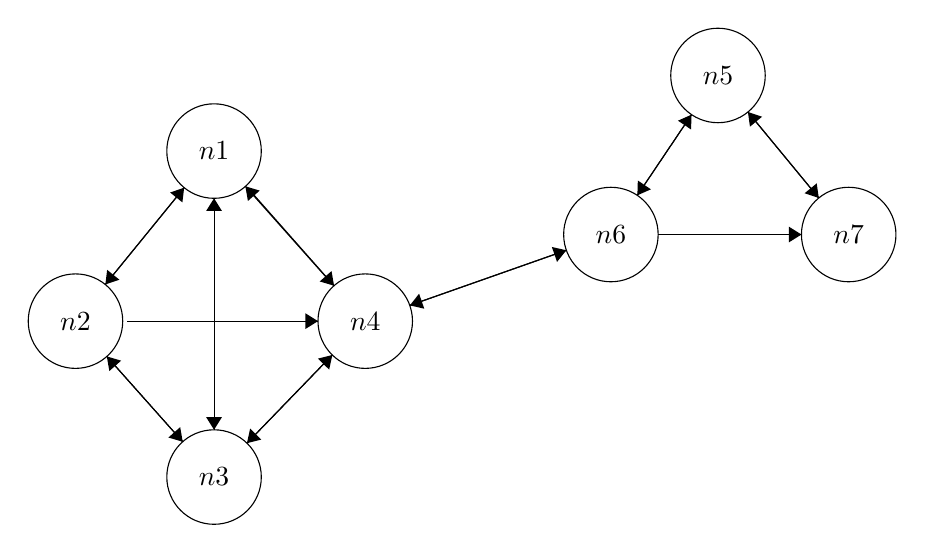
\begin{tikzpicture}[scale=0.2]
\tikzstyle{every node}+=[inner sep=0pt]
\draw [black] (29.1,-13) circle (3);
\draw (29.1,-13) node {$n1$};
\draw [black] (20.3,-23.8) circle (3);
\draw (20.3,-23.8) node {$n2$};
\draw [black] (29.1,-33.7) circle (3);
\draw (29.1,-33.7) node {$n3$};
\draw [black] (38.7,-23.8) circle (3);
\draw (38.7,-23.8) node {$n4$};
\draw [black] (54.3,-18.3) circle (3);
\draw (54.3,-18.3) node {$n6$};
\draw [black] (61.1,-8.2) circle (3);
\draw (61.1,-8.2) node {$n5$};
\draw [black] (69.4,-18.3) circle (3);
\draw (69.4,-18.3) node {$n7$};
\draw [black] (57.3,-18.3) -- (66.4,-18.3);
\fill [black] (66.4,-18.3) -- (65.6,-17.8) -- (65.6,-18.8);
\draw [black] (59.42,-10.69) -- (55.98,-15.81);
\fill [black] (55.98,-15.81) -- (56.84,-15.43) -- (56.01,-14.87);
\draw [black] (67.5,-15.98) -- (63,-10.52);
\fill [black] (63,-10.52) -- (63.13,-11.45) -- (63.9,-10.82);
\draw [black] (27.2,-15.33) -- (22.2,-21.47);
\fill [black] (22.2,-21.47) -- (23.09,-21.17) -- (22.31,-20.54);
\draw [black] (31.19,-31.55) -- (36.61,-25.95);
\fill [black] (36.61,-25.95) -- (35.7,-26.18) -- (36.41,-26.88);
\draw [black] (41.53,-22.8) -- (51.47,-19.3);
\fill [black] (51.47,-19.3) -- (50.55,-19.09) -- (50.88,-20.04);
\draw [black] (31.2,-15.3) -- (36.72,-21.55);
\fill [black] (36.72,-21.55) -- (36.56,-20.62) -- (35.81,-21.28);
\draw [black] (29.1,-16.3) -- (29.1,-30.7);
\fill [black] (29.1,-30.7) -- (29.6,-29.9) -- (28.6,-29.9);
\draw [black] (23.6,-23.8) -- (35.7,-23.8);
\fill [black] (35.7,-23.8) -- (34.9,-23.3) -- (34.9,-24.3);
\draw [black] (22.2,-21.47) -- (27.2,-15.33);
\fill [black] (27.2,-15.33) -- (26.31,-15.63) -- (27.09,-16.26);
\draw [black] (27.11,-31.46) -- (22.29,-26.04);
\fill [black] (22.29,-26.04) -- (22.45,-26.97) -- (23.2,-26.31);
\draw [black] (22.29,-26.04) -- (27.11,-31.46);
\fill [black] (27.11,-31.46) -- (26.95,-30.53) -- (26.2,-31.19);
\draw [black] (29.1,-30.7) -- (29.1,-16);
\fill [black] (29.1,-16) -- (28.6,-16.8) -- (29.6,-16.8);
\draw [black] (36.71,-21.56) -- (31.09,-15.24);
\fill [black] (31.09,-15.24) -- (31.25,-16.17) -- (32,-15.51);
\draw [black] (36.61,-25.95) -- (31.19,-31.55);
\fill [black] (31.19,-31.55) -- (32.1,-31.32) -- (31.39,-30.62);
\draw [black] (51.47,-19.3) -- (41.53,-22.8);
\fill [black] (41.53,-22.8) -- (42.45,-23.01) -- (42.12,-22.06);
\draw [black] (55.98,-15.81) -- (59.42,-10.69);
\fill [black] (59.42,-10.69) -- (58.56,-11.07) -- (59.39,-11.63);
\draw [black] (63,-10.52) -- (67.5,-15.98);
\fill [black] (67.5,-15.98) -- (67.37,-15.05) -- (66.6,-15.68);
\end{tikzpicture}
\end{center}

\end{frame}

\section{Simulation Plots}

\begin{frame}{Simulation Plots}

\begin{figure}[H]
\label{fig:sim1}
  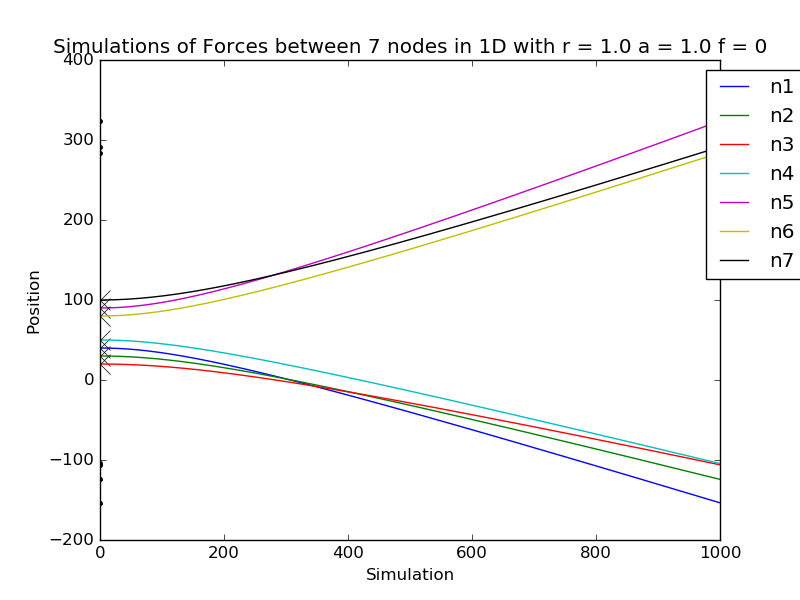
\includegraphics[scale=0.45]{output1.png}
\caption{Simulation of motion of Nodes in 1D}
\end{figure}


\end{frame}


\begin{frame}{Simulation Plots}

\begin{figure}[H]
\label{fig:sim2}
  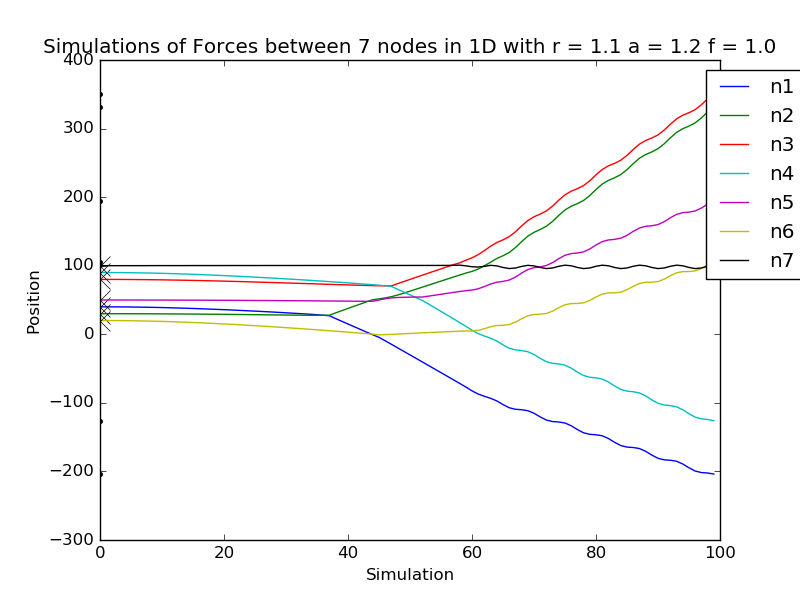
\includegraphics[scale=0.45]{output2.png}
\caption{Simulation of motion of Nodes in 1D}

\end{figure}


\end{frame}

\begin{frame}{Simulation Plots}

\begin{figure}[H]
\label{fig:sim3}
  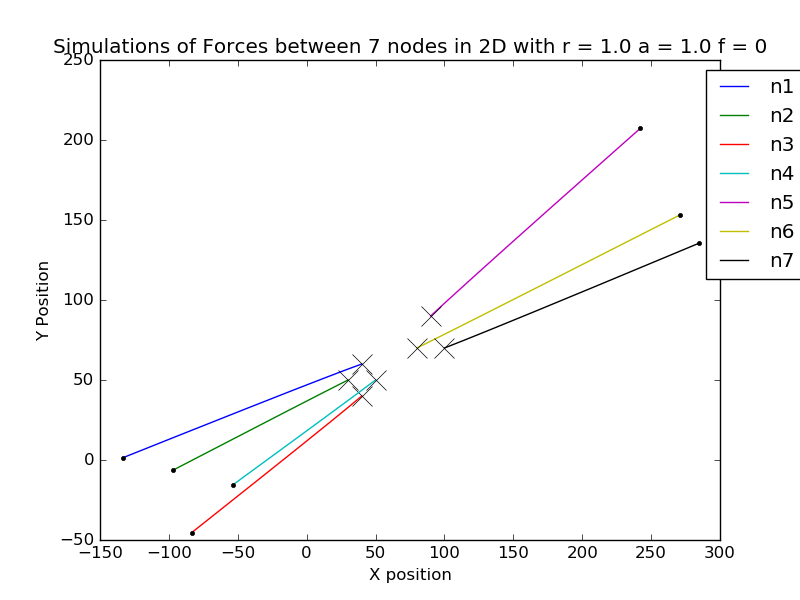
\includegraphics[scale=0.45]{output3.png}
\caption{Simulation of motion of Nodes in 2D}
\end{figure}


\end{frame}

\begin{frame}{Challenged Faced}

\begin{itemize}
    \item As you can see in [\textcolor{blue}{\ref{fig:sim2}}], the cluster (n1,n2,n3,n4) is being split into two because of the presence of another cluster (n5,n6,n7) in the middle. Retaining original clusters is preferable.
    \item Representation in higher dimension is slightly problematic.
    \item There are certain bugs in the code. 
\end{itemize}


\end{frame}


\section{Proposed Methods}
\begin{frame}{Proposed Methods}{}
 \begin{itemize}
     \item Change the laws of attraction \& repulsion i.e instead of inverse of distance squared, we can try with distance squared, this might make further objects come together while not alienating the nearby objects.
     \item Represent distance from origin for each node instead of the position in space. (Might reduce information!!)
     \item (Generalise) Give an edge weight between nodes which can indicate the degree to which they are attracted.
 \end{itemize}
 
\end{frame}


\end{document}


